\documentclass[11pt,a4paper,singlespacing]{article}

%Include file with packages and styles

%%%%%%%%%%%%%%%%%%%%%%%%%%%%%%%%%%%%%%%%%%%%%%%%%%%%%%%%%%%%%%%%%%%%%%%%%%%%%%%
% PACKAGES
%%%%%%%%%%%%%%%%%%%%%%%%%%%%%%%%%%%%%%%%%%%%%%%%%%%%%%%%%%%%%%%%%%%%%%%%%%%%%%%

\usepackage[utf8]{inputenc} 			% Input encoding


%Mathematics
\usepackage{amsmath}					% American Mathematical Society Package
\usepackage{amsfonts}					% Mathematical Fonts
\usepackage{amssymb}					% More mathematical symbols
\usepackage{mathtools}					% More control and better appearence of Mathematics

% Helvetica Font - Optional
%\usepackage{sansmathfonts}
%\usepackage[scaled=0.95]{helvet}
%\renewcommand{\rmdefault}{\sfdefault}
%\usepackage[T1]{fontenc}

%Figures and captions
\usepackage{graphicx}					% More complex version of graphics for figures
\usepackage{caption}					% More control over captions
\usepackage{sidecap}					% Side captions

%ThE LooOks!
\usepackage{fancyhdr}					% Fancy Headers
\usepackage{geometry}					% Control geometry
\usepackage{setspace}

%Tables and other enviorements
\usepackage{tabularx}					% Better tables
\usepackage{booktabs}					% Even better tables
\usepackage{enumitem}					% More control over enumerate enviorements
\usepackage{arydshln}					% Use dashed lines in tables

%Physics
\usepackage{siunitx}					% SI units			
\usepackage{physics}					% Usefull notations ( bras and kets for example)

% Usefull Tools
\usepackage{lipsum}						% Create random text
\usepackage{comment}					% Create comments
\usepackage{hyperref}					% Create hyperlinks
\usepackage{xcolor} 						% Colors
\usepackage{framed}						% Colored frames
\usepackage{setspace}					% Control spaces


%%%%%%%%%%%%%%%%%%%%%%%%%%%%%%%%%%%%%%%%%%%%%%%%%%%%%%%%%%%%%%%%%%%%%%%%%%%%%%%
% DOCUMENT SETUP
%%%%%%%%%%%%%%%%%%%%%%%%%%%%%%%%%%%%%%%%%%%%%%%%%%%%%%%%%%%%%%%%%%%%%%%%%%%%%%%

%Paper Geometry
\geometry{
	paper=a4paper, 	% A4 Paper
	inner=2.5cm, 	% Inner margin
	outer=2.5cm, 	% Outer margin
	top=3cm, 		% Top margin
	bottom=3cm, 	% Bottom margin
}

%Page Style and headers
\pagestyle{fancy}

\renewcommand\headrulewidth{0.4pt}
\renewcommand\footrulewidth{0.4pt}

\lhead{\textbf{Template Report}}
\chead{Main title of your Project }
\rhead{Your Name}
\cfoot{\thepage}
\lfoot{ January 2420}
\rfoot{Professor Name }

%URL links setup
\colorlet{url_blue}{blue!50!black}

\hypersetup{
	pdfpagemode			= {UseOutlines}	,
	bookmarksopen		= true 			,
	bookmarksopenlevel	= 0				,
	hypertexnames		= false			,
	colorlinks			= true			, % Set to false to disable coloring links
	citecolor			= blue			, % The color of citations
	linkcolor			= blue			, % The color of references to document (sections, figures, etc)
	urlcolor			=url_blue		, % The color of hyperlinks (URLs)
	pdfstartview		={FitV}			,
	breaklinks			=true,
	unicode								,
}

%Setup sidecaption
\sidecaptionvpos{figure}{t}

%Set paragraph indentation
\setlength\parindent{10pt}

%Shaded color
\definecolor{shadecolor}{rgb}{0.8,0.8,0.8}

%%%%%%%%%%%%%%%%%%%%%%%%%%%%%%%%%%%%%%%%%%%%%%%%%%%%%%%%%%%%%%%%%%%%%%%%%%%%%%%
% BIBLIO SETUP
%%%%%%%%%%%%%%%%%%%%%%%%%%%%%%%%%%%%%%%%%%%%%%%%%%%%%%%%%%%%%%%%%%%%%%%%%%%%%%%

\usepackage[backend=bibtex , style=chem-angew ,doi=false , url=false , isbn=false ]{biblatex}

%Bibligraphy file
\bibliography{./bib/my_ref} 


% Costumize color of bibliography
\newbibmacro{string+doiurl}[1]{%
	\iffieldundef{doi}
	{\iffieldundef{url}
		{#1}
		{\href{\thefield{url}}{#1}}}
	{\href{https://doi.org/\thefield{doi}}{#1}}}


\makeatletter

\def\blx@driver#1{%
	\ifcsdef{blx@bbx@#1}
	{\usebibmacro{string+doiurl}{\csuse{blx@bbx@#1}}}
	{\ifcsdef{blx@bbx@*}
		{\blx@warning{%
				No driver for entry type '#1'.\MessageBreak
				Using fallback driver}%
			\usebibmacro{string+doiurl}{\csuse{blx@bbx@*}}}
		{\blx@error
			{No driver found}
			{I can't find a driver for the entry type
				'\abx@field@entrytype'\MessageBreak
				and there is no fallback driver either}}}}
\makeatother












\begin{document}
	
%Title
\huge 
\noindent \textbf{Report Title} \\ 
% Name and date
\normalsize
\noindent \textbf{Author:} Your name \\
\noindent \textbf{Date:} January 2420 \\
\normalsize
\vspace{0.4cm}
\hrule

%Summary
\section*{Summary}

%Summary of the Work

Write summary here
 
\vspace{0.4cm}
\hrule

%%%%%%%%%%%%%%%%%%%%%%%%%%%%%%%%%%%%%%%%%%%%%%%%%%%%%%%%%%%%%%%%%%%%%%%%%%%%%%%
% MAIN DOCUMENT
%%%%%%%%%%%%%%%%%%%%%%%%%%%%%%%%%%%%%%%%%%%%%%%%%%%%%%%%%%%%%%%%%%%%%%%%%%%%%%%

\section{Section}


\lipsum[2]

\subsection{Subsection}

\lipsum[1]


%
\begin{equation}
	S   = \int dt L
\end{equation}
%
\lipsum[3] 
%
\begin{equation}
	\frac{d}{dt} \left( \frac{\partial L}{\partial \dot{q}_i} \right) - \frac{\partial L}{\partial q_i} = 0
\end{equation}
%
\lipsum[3]
\begin{equation}
L(t,q_i , \dot{q}_i) \rightarrow \mathcal{L}\left(x_\mu , \phi , \frac{\partial \phi}{\partial x_\mu} \right)
\end{equation}
%
\lipsum[3]
%
\begin{equation}
	S = \int dt L = \int dx^4 \mathcal{L}	
\end{equation}
%
\lipsum[4]
%
\begin{equation}
\partial_\mu \left( \frac{\partial \mathcal{L}}{\partial (\partial_\mu \phi)}\right) - \frac{\partial \mathcal{L}}{\partial \phi} = 0
\end{equation}
%


\begin{SCfigure}[][t]
	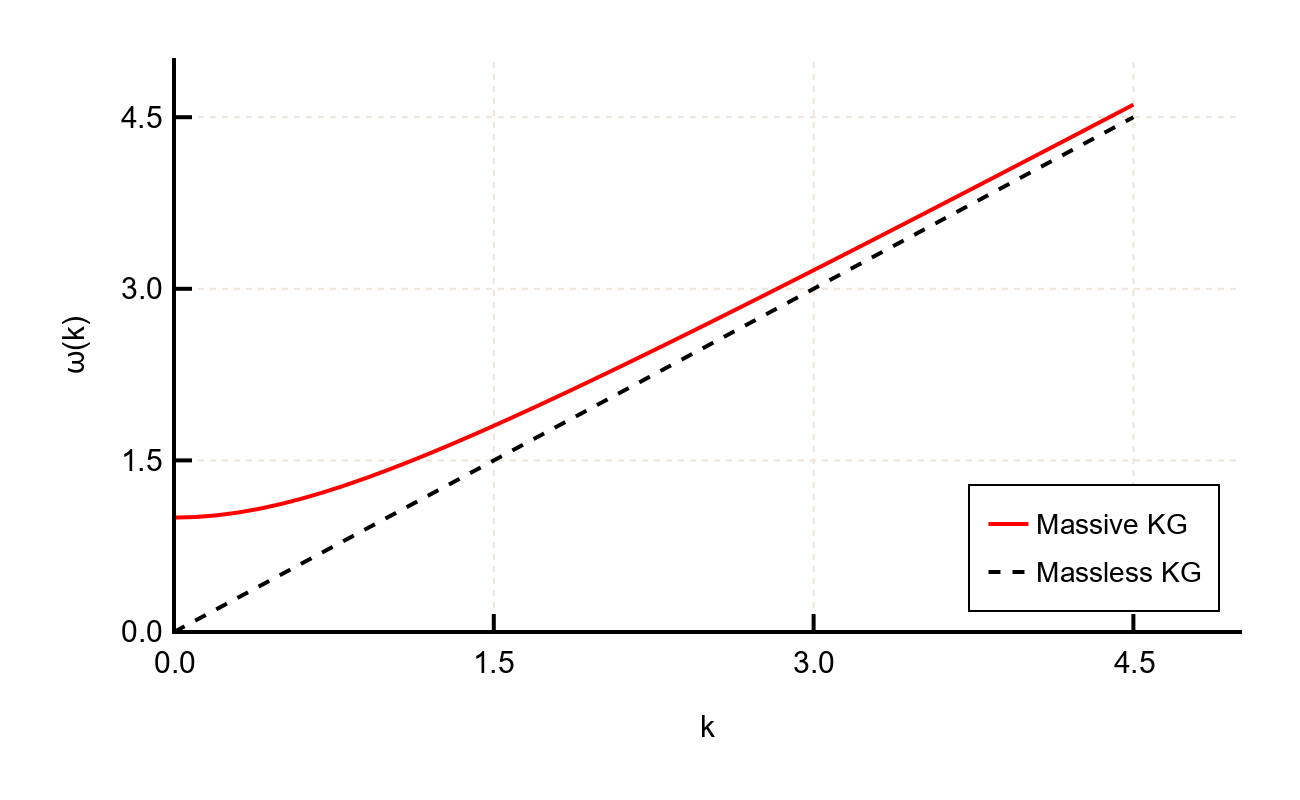
\includegraphics[width=0.8\linewidth]{images/klein_gordon_DR}
	\caption{\protect\rule{0ex}{5ex} 
		This is an example image with a sidecap}
	\label{fig:banana}	
\end{SCfigure}


\subsection{Another Subsection}

\lipsum[1]

\subsubsection*{A Subsection without a number!}


\lipsum[3]

\begin{shaded}
	\textbf{Remark:}
	
	This is a block that can also be used for theorems, small notes...
	%
	\begin{equation}
	\eta_{\mu \nu} = ( - \;,\; + \;,\; + \;,\; +)
	\end{equation}
	
\end{shaded}

\lipsum[3]

\section{Last Section}

\lipsum[2]


\subsection{Example Table}
\lipsum[3]
%
\begin{center}
	\begin{tabular}{ ||p{3cm}|p{3cm}||p{3cm}|p{3cm}||  }
		\hline
		\multicolumn{4}{|c|}{\textbf{Table Title}} \\
		\hline
		\multicolumn{2}{||c||}{\textbf{Group I}} & \multicolumn{2}{c||}{\textbf{Group II}} \\
		\hline
		Parameter 1   	& 	1.0    	& Parameter 3		&   1.0	\\
		Parameter 2   	& 	27.0  	& Parameter 4   	&	0  	\\
		\hline
	\end{tabular}
\end{center}

%\cite{DUMMY:1}

\nocite{*}
\printbibliography

\end{document}